%
% File acl2014.tex
%
% Contact: koller@ling.uni-potsdam.de, yusuke@nii.ac.jp
%%
%% Based on the style files for ACL-2013, which were, in turn,
%% Based on the style files for ACL-2012, which were, in turn,
%% based on the style files for ACL-2011, which were, in turn, 
%% based on the style files for ACL-2010, which were, in turn, 
%% based on the style files for ACL-IJCNLP-2009, which were, in turn,
%% based on the style files for EACL-2009 and IJCNLP-2008...

%% Based on the style files for EACL 2006 by 
%%e.agirre@ehu.es or Sergi.Balari@uab.es
%% and that of ACL 08 by Joakim Nivre and Noah Smith

\documentclass[11pt]{article}
\usepackage{acl2014}
\usepackage{times}
\usepackage{url}
\usepackage{latexsym}
\usepackage{adjustbox}

%\setlength\titlebox{5cm}

% You can expand the titlebox if you need extra space
% to show all the authors. Please do not make the titlebox
% smaller than 5cm (the original size); we will check this
% in the camera-ready version and ask you to change it back.


\title{573 Deliverable 2: A Baseline for Extractive Summarization}

\author{Ayushi Aggarwal  \\
  University of Washington \\
  {\tt ayushiag@uw.edu} \\\And
  Elijah Rippeth \\
  University of Washington \\
  {\tt rippeth@uw.edu} \\\And
  Seraphina Goldfarb-Tarrant \\
  University of Washington\\
  {\tt serif@uw.edu} \\}
  

\date{}

\begin{document}
\maketitle
\begin{abstract}
  We developed an end-to-end extractive text summarization pipeline for the DUC and TAC datasets. We compared three approaches --- first-sentence, random-sentence, and LexRank --- as baselines for future work. We found that the first-sentence approach outperformed random by as much as 50\% in F1 in ROUGE scores and LexRank by as much as 35.4\% in F1 in ROUGE scores, though LexRank generally was judged 
\end{abstract}

\section{Introduction}

Text summarization is the process of compressing a corpus into a compact form with near equivalent saliency. The two main processes by which text summarization is realized are abstractive, which focuses on capturing concepts and generating potentially novel utterances (e.g., paraphrases), and extractive, which filters out the least salient sentences from a corpus, leaving only the most relevant information for a user. \\

In this work, we attempt to develop an end-to-end extractive summarization system for the DUC and TAC summarization tasks. We will explore various summarization approaches and compare their results for use as a baseline for future summarization work.

\section{System Overview}
\subsection{System Architecture}

Our architecture is composed of four main parts:

\begin{enumerate}
\item A configurable corpus reader
\item A preprocessing scheme
\item A configurable summarizer 
\item A post-processing scheme
\end{enumerate}

A wire diagram of the system can be seen below:

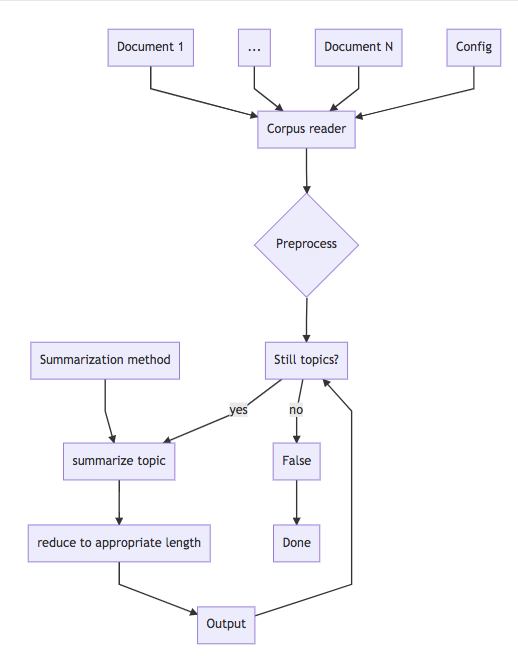
\includegraphics[scale=0.4]{pipeline}


\section{Approach}
The summarization pipeline broadly implements the following functionality:
\subsection{Dataset}
The TAC dataset is categorized by topic, with each topic consisting of a set of multiple documents. Since the task is topic-orientated, our pipeline operates on a subset of topic IDs. It approaches this by storing pointers to docs in the corpus grouped by topic set. This not only allows us to avoid storing the entire doc, which could be perilously expensive for large corpora, but also it allows us to only operate on some subset of the topics covered by our dataset.

In terms of hours, this was probably the most expensive part of the process due to inconsistencies in the formatting of docs in the different datasets. This required separate ingest mechanisms, which proved to be fairly error-prone. 

To make the system slightly more portable, we operated on configuration files from the onset so that members of our system were not married to one specific environment. This proved to be beneficial as each member was able to work both locally and remotely on data. 

\subsection{Preprocessing}
The preprocessing module creates the input for the Content Selection module. Since the documents in a topic are not ordered, we consider them to be a set and create a combined document of all sentences for the topic at hand. All sentences are tokenized before being 
Preprocessing of raw text made use of LXML and BeautifulSoup for XML parsing, and the NLTK Punkt Sentence Tokenizer and TreeBank Word Tokenizer. 


\subsection{Content Selection}
The system baseline takes the sentences for each topic story as the input to the \textbf{summarize} module. 

\subsection{Information Ordering} 
Output of the LexRank score calculator is arranged in descending order of scores. Given the nature of the dataset, we analyzed the possibility of including publishing date for stories. However, since we found the date information to be sparse, temporal information is not incorporated into the information ordering for the final summary.


\subsection{Post-processing}
For each topic within a single document set, a 100-word summary is generated from the LexRank output. We include the highest scoring first \textit{n} sentences that fall within the word-limit. The user can modify the summary word-limit for each topic by resetting the hyper-parameter \textit{word\_num}. 


\section{Results}

For one set of runs, we observed the results shown in Tables 1, 2, and 3.

Overall, we were surprised to see such low ROUGE-1 scores for all of the approaches. Our ROUGE scores were well below those reported in the LexRank paper. Indeed, in stark contrast to the Radev et al. paper, the first-sentences approach outperformed all other approaches in every category apart from ROUGE-1 precision in which LexRank narrowly outperformed the first-sentences approach.\\
In fact, first-sentences and LexRank, though qualitatively different, (as will be discussed below) have very high ROUGE scores with respect to each other. Table 4 shows the impressive level of unigram and even 4-gram overlap between the results of the two systems. For this corpus, selecting the most connected sentences often ends up selecting the first one, though no position information is taken into account.   


\begin{table}[h]
\begin{center}
\begin{tabular}{lp{1cm}p{1cm}p{1cm}}
\hline \bf Type & \bf P & \bf R & \bf F1 \\ \hline
ROUGE-1 & 20.39 & 16.77 & 18.28 \\
ROUGE-2 & 4.37 & 3.69 & 3.98\\
ROUGE-3 & 1.35 & 1.18 & 1.25\\
ROUGE-4 & 0.59 & 0.52 & 0.55 \\
\hline
\end{tabular}
\caption{\label{results-table} Random }
\end{center}
\hspace{2em}

\begin{center}
\begin{tabular}{lp{1cm}p{1cm}p{1cm}}
\hline \bf Type & \bf P & \bf R & \bf F1 \\ \hline
ROUGE-1 & 26.91 & 23.08 & 24.68 \\
ROUGE-2 & 8.13 & 6.99 & 7.46\\
ROUGE-3 & 2.65 & 2.32 & 2.46\\
ROUGE-4 & 1.17 & 1.04 & 1.10 \\
\hline
\end{tabular}
\caption{\label{results-table} First }
\end{center}
\hspace{2em}

\begin{center}
\begin{tabular}{lp{1cm}p{1cm}p{1cm}}
\hline \bf Type & \bf P & \bf R & \bf F1 \\ \hline
ROUGE-1 & 28.95 & 21.98 & 24.75 \\
ROUGE-2 & 7.70 & 5.82 & 6.57\\
ROUGE-3 & 2.49 & 1.91 & 2.14\\
ROUGE-4 & 0.81 & 0.64 & 0.71 \\
\hline
\end{tabular}
\caption{\label{results-table} LexRank}
\end{center}
\hspace{2em}

\begin{center}
\begin{tabular}{lp{1cm}p{1cm}p{1cm}}
\hline \bf Type & \bf P & \bf R & \bf F1 \\ \hline
ROUGE-1 & 52.49 & 51.88 & 51.71 \\
ROUGE-2 & 41.13 & 40.16 & 40.30\\
ROUGE-3 & 36.69 & 35.58 & 35.82\\
ROUGE-4 & 33.87 & 32.77 & 33.01 \\
\hline
\end{tabular}
\caption{\label{results-table} LexRank vs. First }
\end{center}
\end{table}

%%Note: This is a more standard table type when we're comparing multiple different models, but it doesn't really work in double column format so for this version 3 different tables is fine.
% \begin{table}[ht]
% \begin{center}
% \begin{adjustbox}{width=\textwidth/2}
% \begin{tabular}{|r|ccccc|ccccc|ccccc|ccccc|}
%  \hline
%    &&& ROUGE-1 &&&&& ROUGE-2 &&&&& ROUGE-3 &&&&& ROUGE-4 &&\\
%  \hline
%    && A & B & C &&& A & B & C &&& A & B & C &&& A & B & C & \\ \hline
%  Random && A & B & C &&& A & B & C &&& A & B & C &&& A & B & C & \\
%  First && A & B & C &&& A & B & C &&& A & B & C &&& A & B & C & \\
%  Lexrank && A & B & C &&& A & B & C &&& A & B & C &&& A & B & C & \\
 

%  \hline
%  \end{tabular}
%  \end{adjustbox}
%  \end{center}
%  \end{table}


\section{Discussion}
As expected for inverted pyramid structure of Newswire corpus content, the baseline of selecting first-sentences is hard to beat. It was in fact, \textit{harder} to beat than we anticipated, as LexRank does not outperform first-sentences in any area save ROUGE-1 Precision, in which the difference is not large enough to be statistically significant. \\
However, the results were qualitatively different. Many first sentences are a type of short abstract summarizing all topics that follow, but some are a specific appeals to emotion or descriptions of an incident that are meant to introduce the feel of the narrative. For example, in summaries about the repeal of a pharmaceutical drug, some first sentences look like, \textit{When Emily Martin was hospitalized for emergency gallbladder surgery last summer, her doctors found that she had also had acid reflux, causing erosion of her esophagus.} Where \textit{Emily Martin} is not actually important and does not appear later, or in the model summaries, she is there to provide a human element to a broader story. In these cases, another standard narrative convention works \textit{against} the first-sentences heuristic, just as the pyramidal structure works towards it.\\
LexRank avoids this problem by valuing connectedness; these sentences are very detailed, and positionally important, but not very connected.\\
The downside of the LexRank structure is the product of its components. Cosine similarity between sentences will bias towards longer ones, and tf-idf will overweight rare words. Our experiments display this tendency. We extracted statistics on sentence length and on lexical diversity (defined as the ratio of unique to total words, per document) and performed the Mann-Whitney U test on the distributions over the model summaries and the LexRank summaries. We pre-selected $p=0.01$ and found that the difference between both distributions easily passed the significance test. The means of the results are in Table 4. Since the model summaries are drawn from seven separate human summarizers, and are still so consistently shorter in sentence lengths and poorer in lexical diversity, it may be rewarding to look into ways to better approximate the style of human summarizers. That said, it comes with costs - for instance, shorter sentences will require more anaphora and coreference resolution.\\ 
A weakness of all of the baselines is their lack of any kind of discourse coherence, of anaphora resolution, or of penalties for redundancy or paraphrase. As noted, we did not have an ordering component to the system save "best scores" from LexRank. However, ordering would have little effect on ROUGE scores, and had little effect on qualitative evaluation as well. When discourse coherence was lacking, it was not just do to ordering, but to necessary information being missing. Therefore, discourse coherence and anaphora resolution seem more promising areas for future improvement. Methods of event extraction to ensure only one sentence per event, or of distributional semantics to address synonymy, will certainly improve performance qualitatively by reducing redundancy, though it is uncertain what the result will be on ROUGE Recall scores. One simple iterative improvement would be to experiment with addressing redundancy and the bias towards rarity by switching from tf-idf vectors to embedded sentence (or sub-sentence) representations trained on a larger corpus.\\
All baselines also share the weaknesses of their pipeline components, particularly of sentence tokenization. Qualitative analysis revealed some irregularities in sentence tokenization, which may be possible to correct via training a domain specific Punkt Tokenizer. As this is an unsupervised algorithm, this not be prohibitively difficult or expensive.\\
Despite LexRank sentence choices being qualitatively salient, much more so than first-sentences, they did not always display good recall of events/concepts. Of $X$ concepts dispersed amongst the original ten documents (ten per topic), sometimes LexRank will select only a small subset of $X$. For example, in this summarization of a murder, all the details of the actual murder are missing (See Appendix). This is a source of lack of coherence, as there are missing causal links in the chain, and also renders summarizations useless in practice. Summarization as a lossy compression system for transmitting large amounts of information in bitesize pieces should have strong objectives for concept and/or event recall. One of the methods of redundancy, event extraction, could also be used to penalize poor event recall. This will be a necessary metric to add that is algorithm independent.

\begin{table}
\begin{center}
\begin{tabular}{lp{1cm}p{1cm}}
\hline \bf Type & \bf Avg Words & \bf LDR \\ \hline
Model & 20.19 & 0.69 \\
LexRank & 28.25 & 0.73 \\
\hline
\end{tabular}
\caption{\label{results-table} Distributional Statistics. \textbf{Avg Words} are per sentence, \textbf{LDR} is Lexical Diversity Ratio.}
\end{center}
\end{table}

\section{Conclusion}
\label{sec:length}

In this work, we hypothesized that while the first-sentence summary would be a competitive baseline due to the inverse pyramid structure of the data, LexRank would outperform the naive heuristic. Indeed, this was shown to not be the case for our data. The first-sentence baseline outperformed all other baselines in nearly all ROUGE metrics.

We suspect discourse coherence might be improved by penalizing redundancy, which eliminates paraphrases of the same salient topics, improving sentence ordering for chronology, and improving anaphora resolution in output. 


\section*{Acknowledgments}

We would like to specially thank Noam Chomsky, without whom we would likely have no real basis for language. We are eternally indebted to you, Noam.

% include your own bib file like this:
%\bibliographystyle{acl}
%\bibliography{acl2014}

\begin{thebibliography}{}
\bibitem[\protect\citename{Allahyari}2017]{Aho:17}
Allahyari, M., Pouriyeh, S., Assefi, M., Safaei, S., Trippe, E. D., Gutierrez, J. B., and Kochut, K.
\newblock 2017.
\newblock {\em Text summarization techniques: A brief survey.}
\newblock arXiv preprint arXiv:1707.02268.

\bibitem[\protect\citename{Brin and Page}1998]{Aho:98}
Brin, S., Page, L., Motwani, R., and Winograd, T.
\newblock 1998.
\newblock {\em he PageRank citation ranking: Bringing order to the web.}
\newblock Stanford InfoLab.

\bibitem[\protect\citename{Ergan and Radev}2004]{Aho:04}
Erkan, G., and Radev, D. R.
\newblock 2004.
\newblock {\em Lexrank: Graph-based lexical centrality as salience in text summarization.}
\newblock Journal of Artificial Intelligence Research, 22, 457-479.

\bibitem[\protect\citename{Nenkova}2012]{Aho:12}
Nenkova, A., and McKeown, K.
\newblock 2004.
\newblock {\em A survey of text summarization techniques.}
\newblock In Mining text data (pp. 43-76). Springer, Boston, MA.


\end{thebibliography}

\section{Appendix}
\subsection{LexRank Examples}
Note that all of the events of the actual murder are missing.\\
\texttt{critics of prosecutors here said that they had little experience investigating and trying homicides in boulder, a college city that has about one murder a year.\\
at the same time, beckner said he was ``excited ''about new evidence.\\
so when the ramseys had three days of interviews last week with investigators from the district attorney's office, gordon wondered, ``why the wait?\\
the ramsey interviews arrive as boulder, colo., district attorney alex hunter decides whether to take the case to a grand jury.\\
``they may be posturing; they may be trying to help, ''mueller said.}

\end{document}
